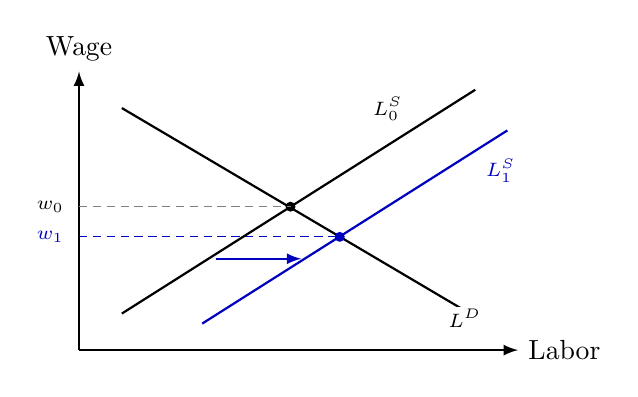
\begin{tikzpicture}[x=0.68cm,y=0.58cm,>=latex]
    \draw[->,thick] (0,0) -- (8.2,0) node[right] {Labor};
    \draw[->,thick] (0,0) -- (0,6.1) node[above] {Wage};

    % Initial labor supply and the fixed MPL schedule (labor demand).
    \draw[thick] (0.8,0.8) -- (7.4,5.7)
        node[pos=0.82,above left=2pt,font=\scriptsize,fill=white,inner sep=1pt] {$L^S_0$};
    \draw[thick] (0.8,5.3) -- (7.3,0.8)
        node[pos=0.88,below right=6pt,font=\scriptsize,fill=white,inner sep=1pt] {$L^D$};

    % The aggregate-demand change shifts labor supply to the right.
    \draw[blue!75!black,thick] (2.3,0.58) -- (8.0,4.81)
        node[pos=0.90,below right=2pt,font=\scriptsize,fill=white,inner sep=1pt] {$L^S_1$};

    \coordinate (EzeroAD) at (3.95,3.14);
    \coordinate (Ead) at (4.87,2.48);
    \fill (EzeroAD) circle (1.8pt);
    \fill[blue!75!black] (Ead) circle (1.8pt);

    \draw[densely dashed,gray] (0,3.14) -- (EzeroAD)
        node[pos=0,left=2pt,font=\scriptsize,text=black] {$w_0$};
    \draw[densely dashed,blue!75!black] (0,2.48) -- (Ead)
        node[pos=0,left=2pt,font=\scriptsize,text=blue!75!black] {$w_1$};
    \draw[->,blue!75!black,thick] (2.55,2.0) -- (4.15,2.0);
\end{tikzpicture}
